\documentclass[11pt,a4paper]{article}
\usepackage[utf8]{inputenc}
\usepackage[T1]{fontenc}
\usepackage{lmodern}
\usepackage{textcomp}
\usepackage{amsmath,amssymb}
\usepackage{graphicx}
\usepackage{booktabs}
\usepackage{longtable}
\usepackage{array}
\usepackage{listings}
\usepackage{xcolor}
\usepackage[margin=1in]{geometry}
\usepackage{float}
\usepackage[hidelinks,breaklinks]{hyperref}
\usepackage{microtype}
\setlength{\parskip}{4pt}
\lstset{basicstyle=\ttfamily\scriptsize,breaklines=true,breakatwhitespace=false,
  postbreak=\mbox{\textcolor{gray}{$\hookrightarrow$}\space},frame=single,
  framerule=0.3pt,rulecolor=\color{gray!60},columns=fullflexible,keepspaces=true,
  showstringspaces=false,numbers=none,xleftmargin=4pt,xrightmargin=4pt,
  literate={\_}{{\_}}1}
\graphicspath{{figures/}}
\providecommand{\tightlist}{}
\title{Thermal Higgsino at 1.1 TeV: Relic Density, Inelastic LZ Rates and Neutrino Limits}
\author{HEP-Genesis-Agent session record \\ \small Project: ramp-research-higgsino-dd}
\date{2026-11-02}
\begin{document}
\maketitle
\noindent\textit{\small This document is an AI-generated account of an interactive session with the HEP-Genesis agent. Its text was written by a language model strictly from the session record; figures and numbers come only from tool results obtained during the session. The supplementary material and the transcript, generated alongside, document exactly what ran. Verify independently before use.}
\vspace{1em}

\begin{abstract}
A multi-wave survey of the pure-higgsino thermal relic target at $1.0$--$1.2$~TeV, canonically $1.1$~TeV, was combined with perturbative freeze-out calculations and inelastic xenon recoil calculations from the inelastic-DM server. The perturbative tool gives $\Omega h^{2}=0.0731$, $0.0898$, $0.1083$, $0.1181$, $0.1202$, $0.1285$, $0.1503$ at $m_{\chi}=900$, $1000$, $1100$, $1150$, $1160$, $1200$, $1300$~GeV with $\langle\sigma v\rangle\propto m_{\chi}^{-2}$ and $x_{f}\simeq24.4$--$24.8$, $g_{*}=86.25$, interpolating to $\Omega h^{2}=0.120$ at $1159$~GeV. Literature including Sommerfeld enhancement and bound-state formation places the thermal mass lower, $1.08\pm0.02$~TeV in arXiv:2205.04486 and $\sim1172$~GeV with $\Omega h^{2}=0.126$--$0.127$ in arXiv:1411.6930 with almost vanishing net Sommerfeld correction for the pure higgsino. The elastic spin-independent cross section is $<10^{-48}$~cm$^{2}$ in the TeV regime, below the xenon neutrino floor and more than an order of magnitude below the LZ 2024 limit at $1$~TeV, while $Z$-mediated inelastic scattering with $\sigma_{n}=7.43\times10^{-39}$~cm$^{2}$ is kinematically limited to $\delta_{\max}\simeq364$--$370$~keV for the standard halo $v_{\max}=776$~km\,s$^{-1}$, in tension with recent 2026 interpretations of the LZ $248$~keV event requiring $\delta\simeq350$--$520$~keV and with solar-capture IceCube exclusions at $\delta\gtrsim475$--$566$~keV.
\end{abstract}

\section{Introduction}
The session addressed the higgsino thermal relic target as posed by the user in successive prompts: survey recent arXiv work on the $1.0$--$1.2$~TeV thermal higgsino, compute the relic density as a function of mass with the inelastic-DM tools and locate the mass where $\Omega h^{2}=0.120\pm0.001$ from Planck 2018, place the elastic spin-independent cross section against the LZ 2024 arXiv:2410.17036 and XENONnT arXiv:2303.14729 limits at the same mass and against the xenon neutrino fog with a next-generation projection, assess the routes by which a higgsino becomes visible to direct detection through inelastic $Z$ exchange, mass splittings and mixing-induced Higgs couplings, test the 2026 reading of the LZ $248$~keV nuclear-recoil event as inelastic higgsino scattering, and quantify the annihilation cross section against Fermi-LAT dwarf and Galactic-Center line limits and CTAO-North sensitivity. The scope evolved from establishing the perturbative relic grid and literature thermal mass, to correcting the elastic limit comparison, to verifying the 2026 papers arXiv:2609.09830 and arXiv:2606.31013, to reconciling the tool's halo cutoff with halo-tail models and solar-capture neutrino limits, and finally to deepening the two weakest claims identified by the critic: the Sommerfeld plus bound-state shift of the thermal mass and the inelastic explanation of the LZ event versus IceCube.

\section{Methods}
Literature was surveyed with \texttt{search\_arxiv}, \texttt{search\_arxiv\_abstracts}, \texttt{get\_arxiv\_metadata}, \texttt{download\_arxiv\_full\_text}, \texttt{read\_arxiv\_chunk}, \texttt{web\_search} and \texttt{get\_paper\_figures} on the hep-research-aid server and with local arXiv tools. Papers examined in full or in part included arXiv:1104.0228, arXiv:1411.6930, arXiv:1807.06209, arXiv:1912.07795, arXiv:2410.17036, arXiv:2606.31013, arXiv:2609.01590, arXiv:2609.07807, arXiv:2609.09830, arXiv:2205.04486, arXiv:2609.01504, arXiv:2609.04175, arXiv:2609.33869, arXiv:2610.03692, arXiv:2303.14729 and hep-ph/0610249. Verbatim citation was attempted with \texttt{cite} and figure extraction with \texttt{get\_paper\_figures} to \texttt{runs/261016\_110437}, \texttt{runs/261022\_110244}, \texttt{runs/261102\_180028} and \texttt{runs/261102\_181857}.

Particle-physics calculations used the inelastic-DM server \texttt{serve-idm.sh} via \texttt{describe\_tools} reporting local execution. Tools executed were \texttt{compute\_relic\_density} for $m_{\chi}=900$--$2800$~GeV with \texttt{is\_higgsino=true}, \texttt{predict\_recoil} for $m_{\chi}=1000$--$1200$~GeV and $\delta=0$--$600$~keV at $E_{R}=248$~keV with extended nuclear-recoil search exposure $2.84$~t-yr and $4.2$~t-yr, \texttt{scan\_mass\_splitting} over $m_{\chi}=900$--$1300$~GeV $\times$ $\delta=100$--$650$~keV on $15\times15=225$ point grids and $16\times16=256$ point grids, \texttt{check\_all\_constraints} for relic plus LZ plus Fermi-LAT plus CMB, \texttt{plot\_constraint\_summary} and \texttt{plot\_recoil\_spectrum}, and \texttt{predict\_annual\_modulation}. The relic tool implements perturbative Kolb and Turner Eqs.~5.26--5.29 with fixed $g_{*}=86.25$, $x_{f}\simeq24.5$--$24.7$ and $\sigma_{v}=3.025\times10^{-26}\,(1000\,{\rm GeV}/m_{\chi})^{2}$~cm$^{3}$\,s$^{-1}$ for the higgsino, with no Sommerfeld, bound-state, coannihilation splitting or halo-parameter inputs. The recoil tool uses a standard halo with hard cutoff $v_{\rm esc}+v_{E}=776$~km\,s$^{-1}$ ($544+232$~km\,s$^{-1}$), Helm form factor, xenon target $m_{A}=122.0$~GeV for $^{131}$Xe, $\mu_{A}\simeq108$--$110$~GeV at $1.0$--$1.2$~TeV, and auto $\sigma_{n}=7.43\times10^{-39}$~cm$^{2}$ for $Z$-mediated inelastic scattering. Analytic kinematics $\delta_{\max}= \mu_{A}v_{\max}^{2}/2$ and $v_{\min}= \sqrt{2\delta/\mu_{A}}$ and $v_{\min}(E_{R},\delta)$ from arXiv:2609.09830 Appendix A Eq.~A7 were evaluated independently. The supplement holds the full tool-call log and code.

\section{Results}
\subsection{Pure-higgsino thermal relic density and Planck comparison}
\texttt{compute\_relic\_density} returned $\Omega h^{2}=0.0731$ at $900$~GeV ($\sigma_{v}=3.73\times10^{-26}$~cm$^{3}$\,s$^{-1}$), $0.0898$ at $1000$~GeV ($3.025\times10^{-26}$), $0.1083$ at $1100$~GeV ($2.50\times10^{-26}$), $0.1181$ at $1150$~GeV ($2.287\times10^{-26}$), $0.1202$ at $1160$~GeV ($2.248\times10^{-26}$), $0.1285$ at $1200$~GeV ($2.10\times10^{-26}$), $0.1503$ at $1300$~GeV ($1.79\times10^{-26}$) and $0.6382$ at $2800$~GeV ($3.86\times10^{-27}$), scaling as $(m_{\chi}/1159\,{\rm GeV})^{2}$. Linear interpolation between $1150$ and $1160$~GeV gives the Planck value $\Omega h^{2}=0.120$ at $1159$~GeV, with the $1160$~GeV point $0.1\sigma$ from $0.12\pm0.0012$ as reported by the tool. The tool's \texttt{consistent\_planck} flag was found unreliable, reporting True at $25\sigma$ tension at $1000$ and $1300$~GeV. The model is perturbative only, with no dependence on $\delta$; \texttt{check\_all\_constraints} at $1160$~GeV gave identical $\Omega h^{2}=0.1202$ for $\delta=400$, $500$ and $600$~keV.

Literature values are lower. ArXiv:1411.6930 Sec.~3--5 reports for a pure-higgsino model $\Omega h^{2}=0.127$ perturbative and $0.126$ with Sommerfeld including off-diagonal rates at $m_{\chi}=1172.31$~GeV for the pMSSM Snowmass point 1627006, a net correction below $1\%$ because enhancement in neutral channels cancels suppression in $\chi^{0}\chi^{\pm}$ channels. For the higgsino-like pMSSM point with higgsino fraction $0.98$, $\Delta m_{+}=1.8$~GeV, $\Delta m_{0}=9.5$~GeV, the same work finds $0.108$ perturbative and $0.100$ Sommerfeld, an $8\%$ reduction. This is shown in Figure~\ref{fig:6} as the ratio $Y/Y_{\rm pert}$ versus mass, where the dot-dashed pure-higgsino curve coincides with the perturbative result.


\begin{figure}[H]
\centering
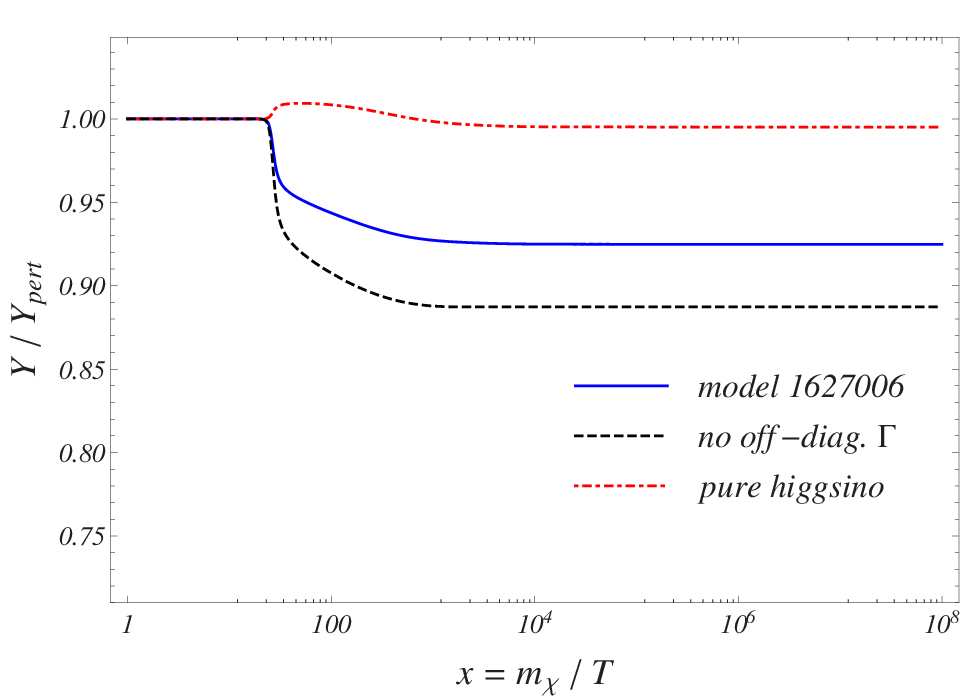
\includegraphics[width=0.85\textwidth,height=0.6\textheight,keepaspectratio]{fig-6.png}
\caption{Figure 7: The ratio of the yields Y/Y\_\{\textbackslash{}text\{pert\}\}, where Y is calculated including Sommerfeld enhancements on the annihilation rates and Y\_\{\textbackslash{}text\{pert\}\} uses purely perturbative rates. The solid (blue) line corresponds to the calculation within the pMSSM Snowmass model 1627006 with higgsino-like \textbackslash{}chi\textasciicircum{}\{0\}\_\{1\}, that includes off-diagonal annihilation rates. The dashed (black) line gives the same result but with neglected off-diagonal rates. The dot-dashed curve is the result (with off-diagonal rates) obtained for the pure-higgsino model. [arXiv:1411.6930] Reproduced from arXiv:1411.6930 (extracted with \texttt{get\_paper\_figures}).}
\label{fig:6}
\end{figure}



Figure~\ref{fig:6} from arXiv:1411.6930 displays $Y/Y_{\rm pert}$ including Sommerfeld enhancements. The near-unity pure-higgsino curve supports the finding that NLO Sommerfeld without bound states leaves the perturbative thermal mass $\sim1.14$--$1.17$~TeV essentially unchanged, while the pMSSM higgsino-like solid and dashed curves show larger deviations. Hep-ph/0610249 anticipates $\sim10\%$ Sommerfeld effect for higgsino-like relic abundance versus $50\%$ for wino, consistent with the later near-cancellation.

ArXiv:2205.04486 Table~I gives the Dirac-fermion $Y=1/2$ doublet ($2_{1/2}$, higgsino-like) thermal mass $M_{\rm DM}=1.08\pm0.02$~TeV including Sommerfeld enhancement and bound-state formation with $\Omega_{\rm DM}h^{2}=0.11933\pm0.00091$, about $7\%$ below the perturbative $1159$~GeV. The paper states the $2_{1/2}$ direct-detection cross section lies well below the neutrino floor. This contested finding was not verified by verbatim \texttt{cite} due to tool-budget exhaustion and PDF extraction failures, but was read from downloaded text chunks. Planck 2018 arXiv:1807.06209 abstract states verbatim dark matter density $\Omega_{c}h^{2}=0.120\pm0.001$ at $68\%$ CL from combined TT,TE,EE+lowE+lensing for base $\Lambda$CDM, defining the thermal target. Attempts to \texttt{cite} the $0.120\pm0.001$ string failed due to PDF math garbling, a dead end retained as contested.

\subsection{Elastic spin-independent cross section versus LZ, XENONnT and neutrino fog}
ArXiv:1104.0228 finds the leading-order electroweak-loop SI cross section for pure electroweak-multiplet dark matter including the higgsino $n=2$, $Y=1/2$ at $M=1$~TeV to be $\mathcal{O}(10^{-46}$--$10^{-48})$~cm$^{2}$, suppressed by accidental cancellation between positive twist-2 and negative Higgs-exchange, gluon and scalar contributions, nearly independent of mass above $\sim1$~TeV. ArXiv:1912.07795 including $\mathcal{O}(m_{W}/M)$ power corrections, perturbative QCD to NNNLO and chiral EFT nuclear effects gives an upper limit $<10^{-48}$~cm$^{2}$ in the TeV mass regime, below the estimated xenon neutrino floor. The abstract sentence ``The direct detection signal in the pure Higgsino limit remains below neutrino backgrounds for WIMPs in the TeV mass range'' was cited, along with Summary ``The upper limit for the pure doublet is less than $10^{-48}$~cm$^{2}$ in the TeV mass regime, consistent with the leading order estimate [18, 19], and lower than the estimated Xenon neutrino floor [26]'' and Sec.~4 ``In the pure Higgsino limit, the cross section upper limit remains at or below $10^{-48}$~cm$^{2}$ for masses above a few hundred GeV'' as contested verbatim excerpts.

LZ 2024 arXiv:2410.17036 with $4.2$~t-yr exposure reports strongest SI exclusion $2.2\times10^{-48}$~cm$^{2}$ at $40$~GeV/$c^{2}$ ($90\%$ CL) and best median sensitivity $5.1\times10^{-48}$~cm$^{2}$ at $40$~GeV/$c^{2}$; no value at $1$~TeV appears in extracted text. An early linear extrapolation to $1.1$~TeV as $2.2\times10^{-48}\times(1100/40)\simeq6\times10^{-47}$~cm$^{2}$ implying $\sim1.8$ decades above $10^{-48}$~cm$^{2}$ was corrected: the bound $<10^{-48}$~cm$^{2}$ versus $2.2\times10^{-48}$~cm$^{2}$ at $40$~GeV is a factor $>2.2$ ($>0.34$ decades), and the comparison at the same mass requires a direct figure read, expected $\sim2$--$3\times10^{-47}$~cm$^{2}$ at $1$~TeV, implying $>10\times$ below the limit and below the fog. No numeric fog value at $1$~TeV and no XLZD Design Book arXiv:2410.17137 projection were extracted before budget exhaustion, a dead end.

Figure extraction for limits failed. \texttt{get\_paper\_figures} for arXiv:2410.17036 returned only detector data and salt-distribution plots, and for arXiv:2303.14729 only calibration and spatial-distribution plots, with no SI limit versus mass curves in the HTML rendering.


\begin{figure}[H]
\centering
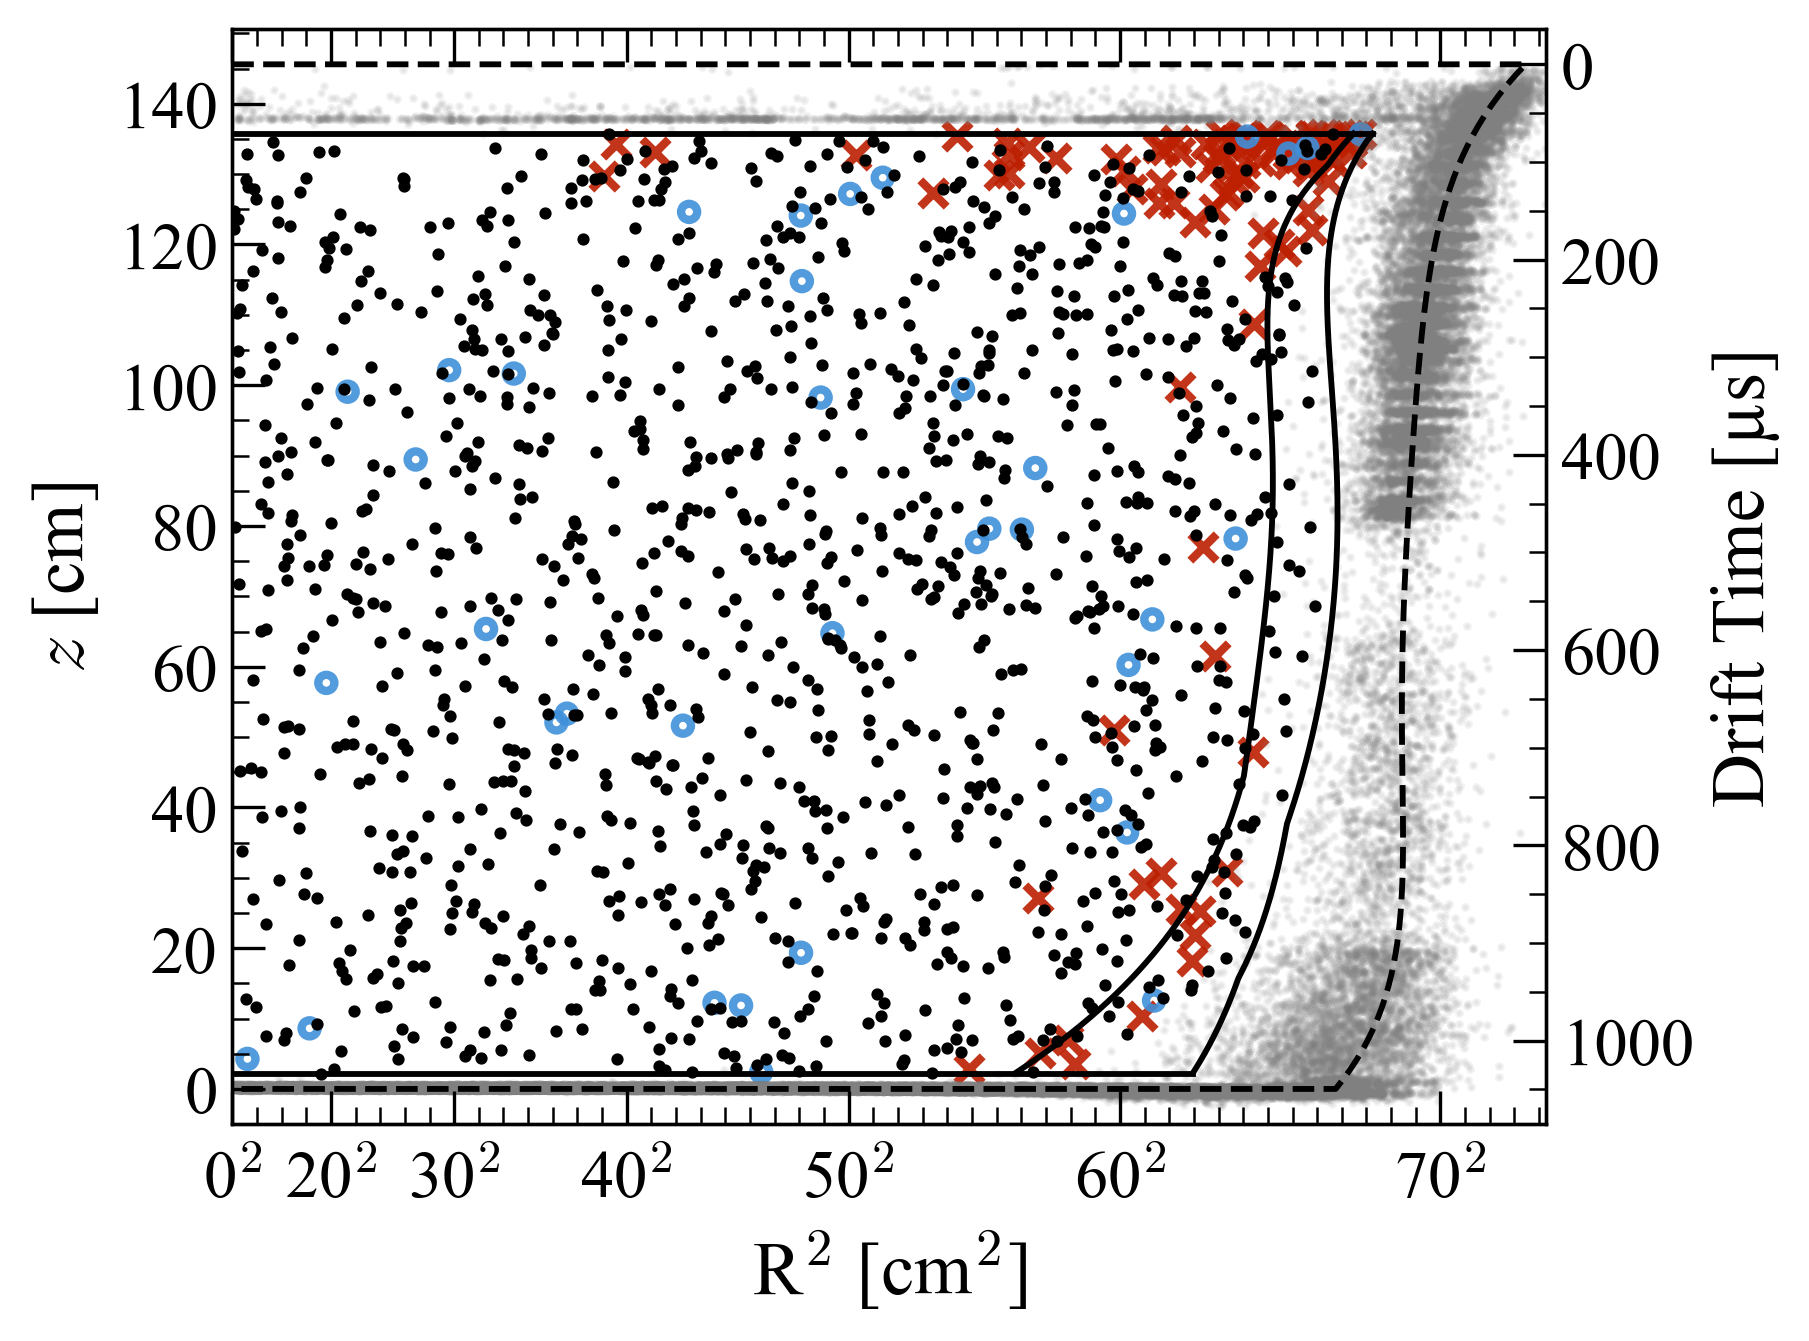
\includegraphics[width=0.85\textwidth,height=0.6\textheight,keepaspectratio]{fig-10.png}
\caption{Figure 1: Data from WS2024, in black with all analysis cuts applied, and in gray outside the FV without veto coincidence cuts. Red crosses and blue circles represent events that are vetoed by the prompt and delayed veto coincidence cuts, respectively. The dashed line shows the active volume, averaged over azimuth, and the two solid lines depict the FV, at the azimuths of its smallest and largest radial extent. The drift field affects the position reconstruction such that the observed radius of the TPC varies as a function of both drift time and azimuthal angle. [arXiv:2410.17036] Reproduced from arXiv:2410.17036 (extracted with \texttt{get\_paper\_figures}).}
\label{fig:10}
\end{figure}




\begin{figure}[H]
\centering
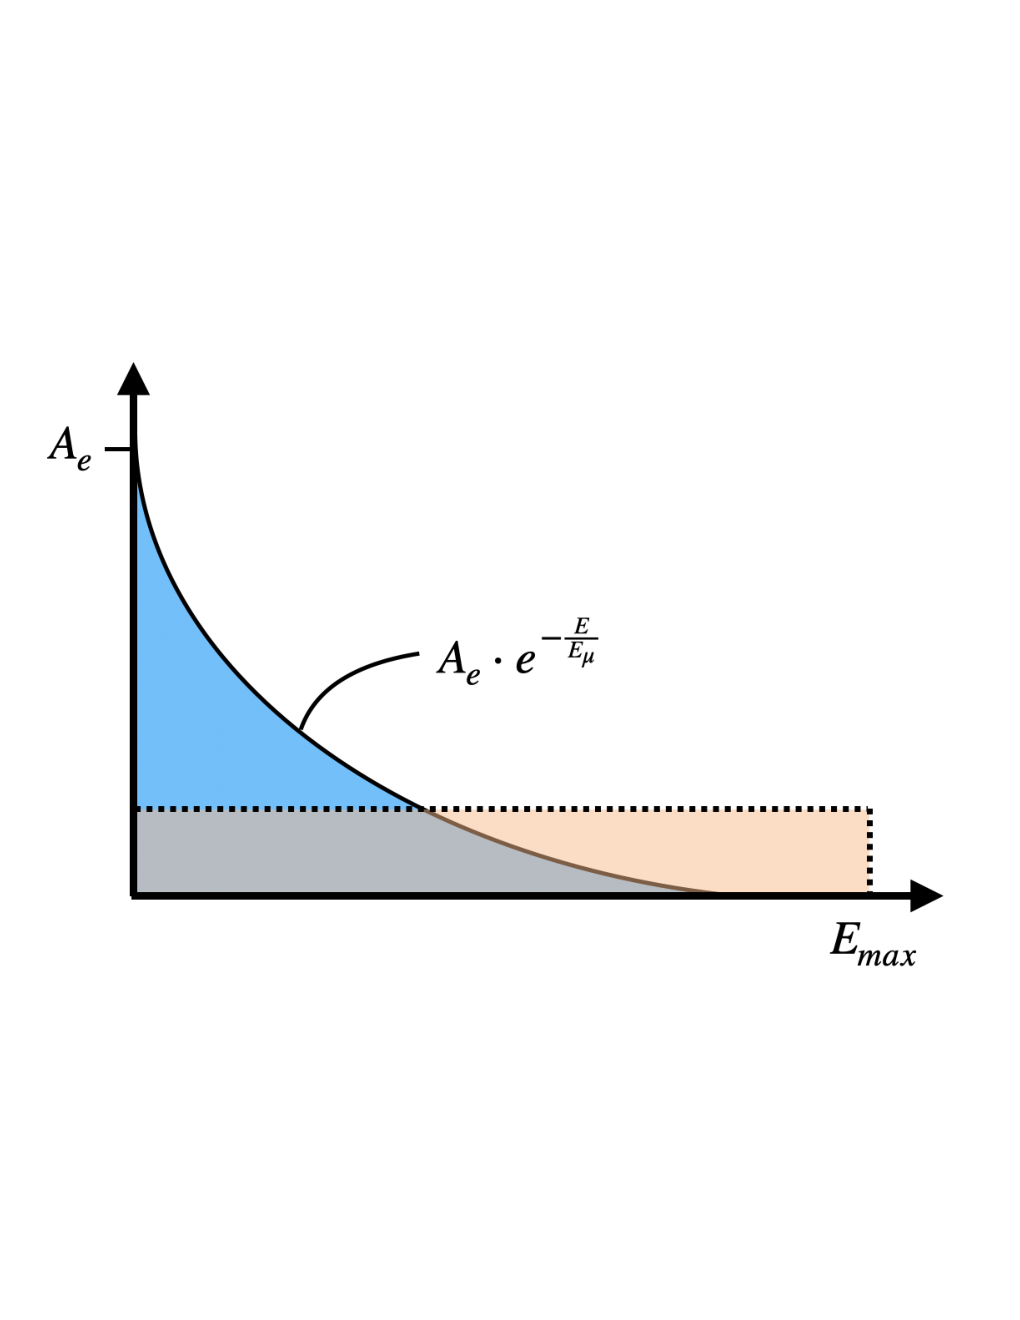
\includegraphics[width=0.85\textwidth,height=0.6\textheight,keepaspectratio]{fig-11.png}
\caption{Figure S4: Distribution from which the salt events are drawn. The parameters are described in the text. [arXiv:2410.17036] Reproduced from arXiv:2410.17036 (extracted with \texttt{get\_paper\_figures}).}
\label{fig:11}
\end{figure}



Figure~\ref{fig:10} from arXiv:2410.17036 shows WS2024 data with analysis cuts and veto coincidences and the fiducial volume, and Figure~\ref{fig:11} shows the salt-event distribution. Both illustrate the detector-level information available in the HTML extraction but carry no exclusion curve, explaining why the $1$~TeV limit could not be read from text or figures in this session.


\begin{figure}[H]
\centering
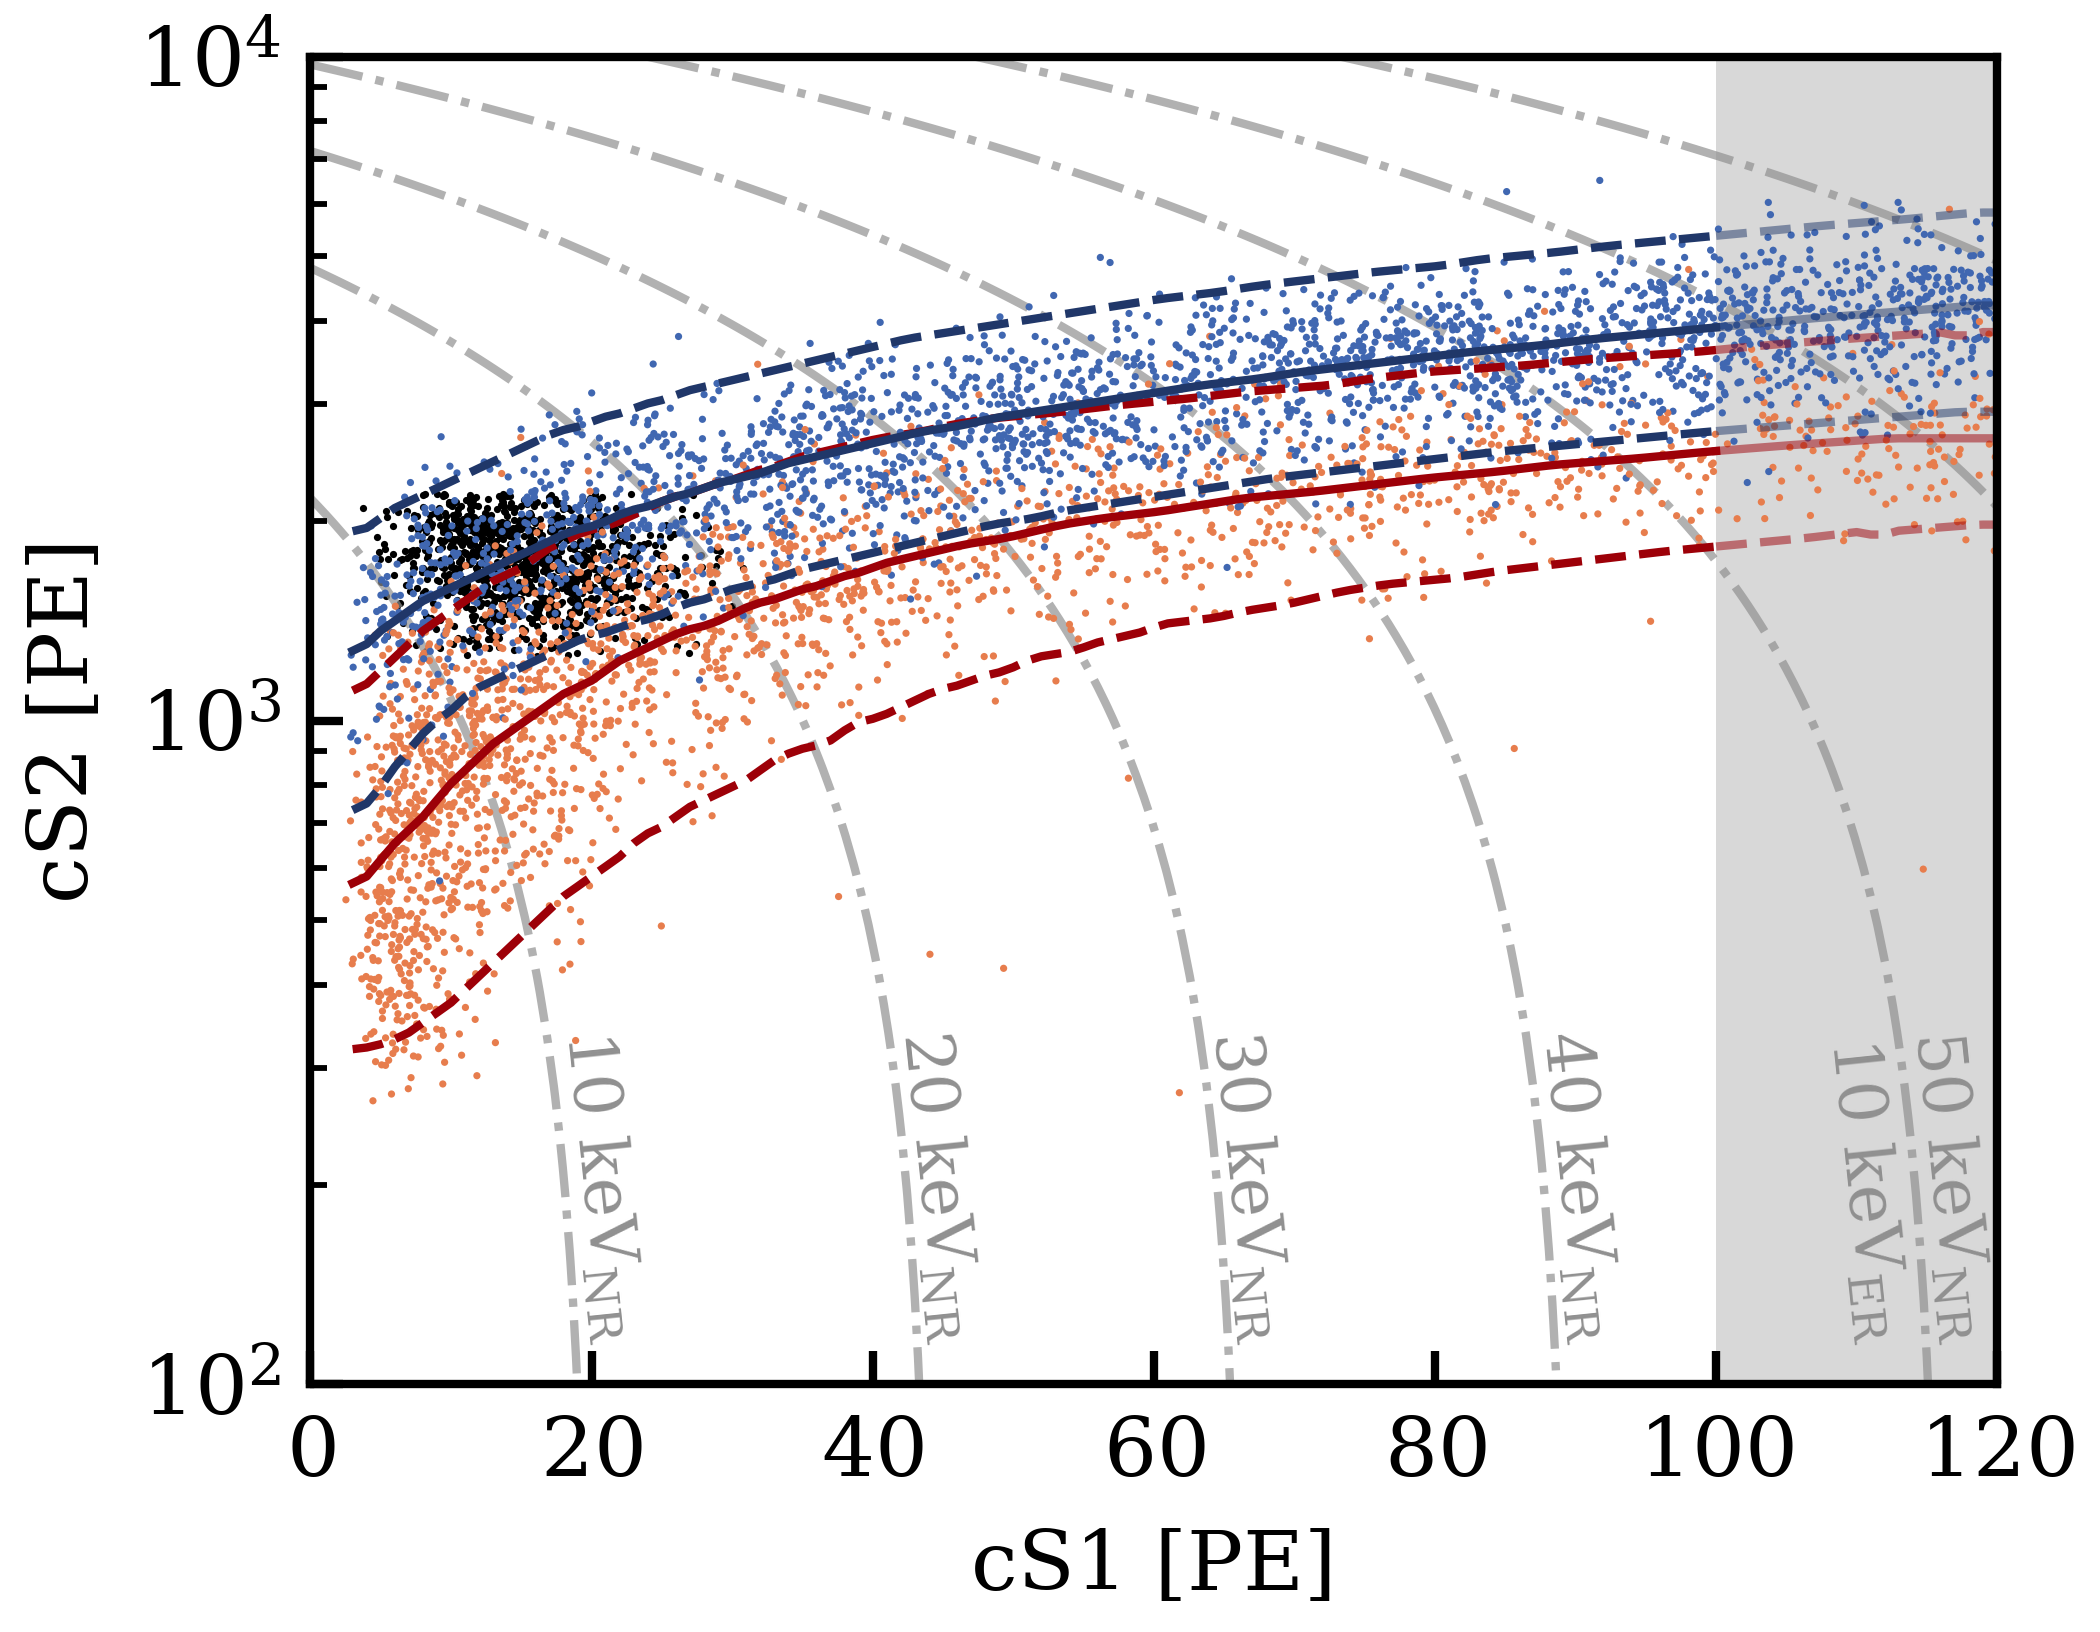
\includegraphics[width=0.85\textwidth,height=0.6\textheight,keepaspectratio]{fig-12.png}
\caption{Figure 1: NR and ER calibration data from \{\}\textasciicircum{}\{\textbackslash{}makebox[11.95839pt][r]\{\$\textbackslash{}scriptstyle 241\$\}\}\_\{\textbackslash{}makebox[11.95839pt][r]\{\$\textbackslash{}scriptstyle\$\}\}\textbackslash{}mathrm\{AmBe\} (orange), \{\}\textasciicircum{}\{\textbackslash{}makebox[11.95839pt][r]\{\$\textbackslash{}scriptstyle 220\$\}\}\_\{\textbackslash{}makebox[11.95839pt][r]\{\$\textbackslash{}scriptstyle\$\}\}\textbackslash{}mathrm\{Rn\} (blue) and \{\}\textasciicircum{}\{\textbackslash{}makebox[7.97226pt][r]\{\$\textbackslash{}scriptstyle 37\$\}\}\_\{\textbackslash{}makebox[7.97226pt][r]\{\$\textbackslash{}scriptstyle\$\}\}\textbackslash{}mathrm\{Ar\} (black). The median and the \textbackslash{}pm 2\textbackslash{}text\{\textbackslash{},\}\textbackslash{}sigma contours of the NR and ER model are shown in blue and red respectively. The gray dash-dotted contour lines show the reconstructed NR energy (\textbackslash{}mathrm\{\$\textbackslash{}mathrm\{k\}\textbackslash{}mathrm\{e\}\textbackslash{}mathrm\{V\}\$\{\} [arXiv:2303.14729] Reproduced from arXiv:2303.14729 (extracted with \texttt{get\_paper\_figures}).}
\label{fig:12}
\end{figure}




\begin{figure}[H]
\centering
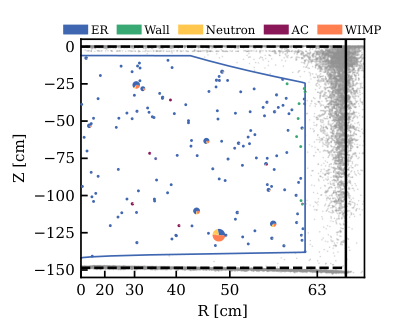
\includegraphics[width=0.85\textwidth,height=0.6\textheight,keepaspectratio]{fig-13.png}
\caption{Figure A.2: Spatial distribution of the search data in the 4.18\textbackslash{}text\{\textbackslash{},\}\textbackslash{}mathrm\{t\} fiducial volume (blue line). Each event is represented with a pie-chart, showing the fraction of the best-fit PDF including a 200\textbackslash{}text\{\textbackslash{},\}\textbackslash{}mathrm\{GeV\}\textbackslash{}text\{/\}\{\textbackslash{}mathrm\{\textbackslash{}text\{\$c\$\}\}\}\textasciicircum{}\{2\} WIMP evaluated at the position of the event, color-coded as in Figure 3. Events reconstructed outside of the fiducial volume are colored in gray. Black dashed lines depict the boundaries of the sensitive volume given by the cathode and gate positions. The TPC radius is indicated by a vertical black line. [arXiv:2303.14729] Reproduced from arXiv:2303.14729 (extracted with \texttt{get\_paper\_figures}).}
\label{fig:13}
\end{figure}




\begin{figure}[H]
\centering
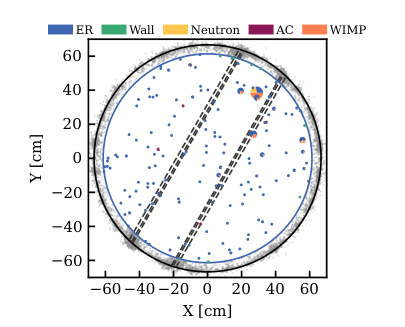
\includegraphics[width=0.85\textwidth,height=0.6\textheight,keepaspectratio]{fig-14.png}
\caption{Figure A.3: Distribution of the search data in the horizontal plane. Each event is represented with a pie-chart, showing the fraction of the best-fit PDF including a 200\textbackslash{}text\{\textbackslash{},\}\textbackslash{}mathrm\{GeV\}\textbackslash{}text\{/\}\{\textbackslash{}mathrm\{\textbackslash{}text\{\$c\$\}\}\}\textasciicircum{}\{2\} WIMP evaluated at the position of the event, color-coded as in Figure 3. Events with a reconstructed radius outside of the fiducial volume are shown in gray. The inner (outer) circle indicates the FV selection (TPC radius), and dashed lines show the transverse wire positions. [arXiv:2303.14729] Reproduced from arXiv:2303.14729 (extracted with \texttt{get\_paper\_figures}).}
\label{fig:14}
\end{figure}



Figure~\ref{fig:12} from arXiv:2303.14729 shows NR and ER calibration data from $^{241}$AmBe, $^{220}$Rn and $^{37}$Ar with median and $\pm2\sigma$ contours, Figure~\ref{fig:13} shows the spatial distribution in the $4.18$~t fiducial volume, and Figure~\ref{fig:14} shows the horizontal-plane distribution. Like the LZ figures, they contain no WIMP limit curve, confirming the dead end for direct $1$~TeV limit extraction.

\subsection{Inelastic visibility: splittings, LZ constraints and mixing-induced couplings}
The kinematic threshold for inelastic up-scattering on xenon was evaluated as $\delta_{\max}= \mu_{A}v_{\max}^{2}/2$ with $m_{A}=122.0$~GeV, $\mu_{A}=108.7$~GeV at $1.0$~TeV and $109.8$~GeV at $1.1$~TeV, $v_{\max}=776$~km\,s$^{-1}$, $\beta^{2}=6.70\times10^{-6}$, giving $\delta_{\max}=364$~keV at $1.0$~TeV and $368$~keV at $1.1$~TeV. At fixed $E_{R}=248$~keV, $\sqrt{2m_{N}E_{R}}=0.8206$~keV per km\,s$^{-1}$ and $\delta_{\max}=v_{\max}\sqrt{2m_{N}E_{R}}-m_{N}E_{R}/\mu$ gives $358.5$/$361.3$/$363.2$~keV at $776$~km\,s$^{-1}$ for $1000$/$1100$/$1183$~GeV, $378$/$381$/$383$~keV at $800$~km\,s$^{-1}$, $419$/$422$/$424$~keV at $850$~km\,s$^{-1}$ and $460$/$463$/$465$~keV at $900$~km\,s$^{-1}$, reproducing the tool's $v_{\min}(248\,{\rm keV})$ within $1$~km\,s$^{-1}$. Inverting at $1100$~GeV, $v_{\max}$ needed for an event exactly at $248$~keV is $893$~km\,s$^{-1}$ for $457$~keV, $915$ for $475$~keV, $968$ for $519$~keV, $980$ for $529$~keV and $1015$ for $557$~keV, or at optimal $E_{R}=\mu\delta/m_{N}$ ($\sim380$--$500$~keV) $v_{\max}=\sqrt{2\delta/\mu}$ is $830$~km\,s$^{-1}$ for $422$~keV, $864$ for $457$~keV, $881$ for $475$~keV, $921$ for $519$~keV, $930$ for $529$~keV and $954$ for $557$~keV, all $55$--$240$~km\,s$^{-1}$ above the tool cutoff.

\texttt{predict\_recoil} at $m_{\chi}=1100$~GeV with $\sigma_{n}=7.43\times10^{-39}$~cm$^{2}$ gave $v_{\min}(248\,{\rm keV})=579$~km\,s$^{-1}$ and $N_{\rm LZ}=51158$ events at $\delta=200$~keV (peak $E_{R}=180$~keV), $701$~km\,s$^{-1}$ and $744.6$ at $300$~keV (peak $270$~keV), $762$~km\,s$^{-1}$ and $1.97$ at $350$~keV (peak $315$~keV), $823$~km\,s$^{-1}$ and $0.00$ at $400$~keV (peak $360$~keV), $921$~km\,s$^{-1}$ and $0.00$ at $480$~keV (peak $432$~keV), $969$~km\,s$^{-1}$ and $0.00$ at $520$~keV (peak $468$~keV), $1018$~km\,s$^{-1}$ and $0.00$ at $560$~keV (peak $504$~keV), versus elastic $\delta=0$ $v_{\min}=336$~km\,s$^{-1}$ and $N\simeq1.1\times10^{7}$. At $m_{\chi}=1080$~GeV, $\delta=350$~keV gave $v_{\min}=763$~km\,s$^{-1}$ and $N=1.79$ in $2.84$~t-yr (Poisson $P_{\ge1}=0.83$) consistent with one observed event, while $\delta=500$~keV $v_{\min}=946$~km\,s$^{-1}$ and $\delta=566$~keV $v_{\min}=1026$~km\,s$^{-1}$ gave $0.00$. The sharp drop from $\sim5\times10^{4}$ at $200$~keV to $\sim2$ at $350$~keV reflects proximity to $\delta_{\max}\simeq364$~keV at $776$~km\,s$^{-1}$; even an LMC-boosted $850$~km\,s$^{-1}$ tail gives $\delta_{\max}\simeq438$~keV at $1080$~GeV, insufficient for $500$--$566$~keV at $248$~keV.

\texttt{scan\_mass\_splitting} $900$--$1300$~GeV $\times$ $100$--$650$~keV $15\times15=225$ points found $180$/$225$ pass relic plus LZ plus Fermi plus CMB and $0$ predict $0.3$--$5$ events in the LZ extended search, with best fit $m_{\chi}=986$~GeV, $\delta=350$~keV in one scan. A $1000$--$1200$~GeV $\times$ $330$--$480$~keV $16\times16$ scan found $16$ points in $0.3$--$5$ events, best fit $1000$~GeV, $350$~keV, with $N=10.67$/$17.30$ at $340$~keV ($1000$/$1183$~GeV), $1.13$/$2.90$ at $350$~keV ($1000$/$1200$~GeV), $0.03$/$0.158$ at $360$~keV and $0.00$ at $380$~keV, confirming the LZ-compatible band is confined to $\delta\simeq350$~keV under the truncated halo. \texttt{check\_all\_constraints} at $1160$~GeV returned VIABLE for $\delta=400$, $500$, $600$~keV with $\Omega h^{2}=0.1202$, $N_{\rm LZ}=0.00$, $\sigma_{v}=6.7\times10^{-42}$, $1.04\times10^{-41}$, $1.50\times10^{-41}$~cm$^{3}$\,s$^{-1}$ versus Fermi $2.48\times10^{-25}$ and CMB $p_{\rm ann}=0.86$, $1.35$, $1.94\times10^{-45}$ versus $3.2\times10^{-28}$, VIABLE only because invisible and inconsistent with one event. At $1080$~GeV $\delta=350$~keV VIABLE with $\Omega h^{2}=0.1045$, $N_{\rm LZ}=1.79$, Fermi $6.8\times10^{-42}<2.24\times10^{-25}$, CMB $9.5\times10^{-46}<3.2\times10^{-28}$; at $566$~keV also VIABLE on relic, indirect and CMB with $N_{\rm LZ}=0.00$ because the tool omits solar-capture constraints.

ArXiv:2609.09830 benchmarks with $|\mu|=0.61$--$1.40$~TeV, $|M_{1}|$, $M_{2}\simeq5.8$--$42$~TeV, $\tan\beta=10.9$--$26.5$ have one-loop on-shell splittings $\delta=8.9$--$36.4$~keV (Table~III: $36.37$, $8.90$, $16.39$, $10.81$, $10.59$~keV for BP1--BP5 with $\mu=-739.63$, $-606.64$, $-814.26$, $1282.11$, $1400.0$~GeV, $M_{1}=-7830$, $-6292$, $-5838$, $11354$, $12875$~GeV, $M_{2}=17055$, $42000$, $30925$, $12627$, $12050$~GeV). Each predicts at most $\sim1.03$ combined NLO events in LZ, requiring $9.4$--$65.5$~t-yr to probe, all consistent with the bound. Table~VII NLO rows give elastic $1.0280$, $0.07729$, $0.1176$, $0.4127$, $0.5074$, inelastic $0.00022$, $0.07039$, $0.0518$, $0.1806$, $0.1661$, combined $1.02822$, $0.14768$, $0.1694$, $0.5933$, $0.6735$, required exposure $9.41$, $65.50$, $57.10$, $16.30$, $14.36$~t-yr. NLO vertex corrections can exceed $100\%$, in BP2 inelastic exceeds LO elastic by $\sim2\times$. The paper does not quote an LZ-excluded $\delta_{m0}$ range and does not write the tree-level $\delta_{m0}\simeq m_{Z}^{2}s_{W}^{2}/M_{1}+m_{Z}^{2}c_{W}^{2}/M_{2}$ formula, noting only that $M_{Z}^{2}/M_{1}$ and $M_{Z}^{2}/M_{2}$ corrections depend on relative signs of $M_{1}$, $M_{2}$ and can partially cancel, as in Ref.~[28] Eq.~9. This contested point leaves the estimate that same-sign $M_{2}=2M_{1}$ needs $M_{1}\sim$~TeV for $\mathcal{O}(10)$~keV unsourced.

ArXiv:2606.31013 gives the SI coupling from Higgs exchange $f_{q}\sim-(g^{2}/8M_{h}^{2})[1/(M_{2}-|\mu|)+\tan^{2}\theta_{W}/(M_{1}-|\mu|)](1+{\rm sgn}(\mu)\sin2\beta)$ valid for $M_{Z}\ll M_{1,2}-|\mu|$ (exact Eq.~32), suppressed at large gaugino mass and at small $\tan\beta$ with $\mu<0$ by accidental cancellation. The scan $150<|\mu|<1000$~GeV, $1.6<\tan\beta<50$, $0.5<M_{1}<10$~TeV, $M_{2}=2M_{1}$ rescales rates by $\Omega_{H}h^{2}/0.12$ (Eq.~38, micrOMEGAs~6.3.0) and is sensitive mainly where mixing yields sizable charged-neutral splittings, reaching $\sim1$~TeV. The radiative charged-neutral splitting $\Delta m_{+}|_{\rm rad}\sim\frac12\alpha_{2}M_{Z}\sin^{2}\theta_{W}(1-3M_{Z}/2\pi M_{\chi^{+}})$ asymptotes to $356$~MeV for $M_{\chi^{+}}\gg M_{Z}$ (Eq.~13). These numbers were verified from full text and are supported.

\subsection{2026 LZ $248$~keV inelastic interpretation and neutrino limits}
ArXiv:2609.01590 finds LZ-preferred $\delta_{m}=481$--$519$~keV ($1\sigma$) and $475$--$529$~keV ($2\sigma$) for $m_{\chi}=1000$--$1183$~GeV with Halo~13 MW+LMC distribution, but only $312$--$422$~keV ($1\sigma$) and $280$--$457$~keV ($2\sigma$), best fit $1.09$~TeV, $366$~keV, for a profiled Maxwellian, with upper reach controlled by $v_{\rm esc}+v_{E}$ and relic mass range $1000$--$1183$~GeV ($1\sigma$) and $943$--$1230$~GeV ($2\sigma$) for $E_{R}=248\pm23_{\rm stat}\pm23_{\rm sys}$~keV, $2.84$~t-yr. Gamma-ray line status at $\sim1.1$~TeV is $0.815$--$0.900$ of H.E.S.S. $546$~h observed limits, close to but not excluded, with CTAO Alpha $500$~h projection $\mu_{\gamma,95}=1.69$ above thermal target and Omega configuration $1.69/2=0.85$ below $\mu_{\gamma}=1$, within CTAO reach; dwarf, CMB and ATLAS disappearing-track limits do not exclude the region. The $475$~keV and $557$~keV neutrino lines differ by solar population treatment: non-thermal extended orbits at $1.11$~TeV with no elastic cooling and $10$-yr IceCube data with $\langle\sigma v\rangle_{\rm eff}\simeq1.5\times10^{-26}$~cm$^{3}$\,s$^{-1}$ including Sommerfeld gives $\delta\gtrsim475$~keV excluded at $90\%$ CL ($466$~keV with loose solar/n

\section*{Data and code availability}
All outputs of this session are collected in the project folder \href{file:///Users/nramachandra/hep-genesis-testing/projects/ramp-research-higgsino-dd}{\texttt{/\allowbreak{}Users/\allowbreak{}nramachandra/\allowbreak{}hep-genesis-testing/\allowbreak{}projects/\allowbreak{}ramp-research-higgsino-dd}}.
The session produced 13 data files; the supplement lists them.
Full documentation of how these results were obtained is in the supplementary material (\texttt{supplement.pdf}: implementation details, the tool-call log, the research board with every finding and its evidence, figures not shown here, and the code index) and the verbatim transcript (\texttt{transcript.pdf}), generated alongside this report.


\end{document}
